\documentclass[article,A4,12pt]{llncs}
\usepackage[T1]{fontenc}
\usepackage{amsmath}
\usepackage{amssymb}
\usepackage{amsfonts}
\usepackage{mathrsfs, bm}

\usepackage{graphicx}
\usepackage{tabularx}
\usepackage{subfig}
\usepackage{epsf,times}
\usepackage{color}
\usepackage{wrapfig}
\usepackage{cases}
\usepackage{multicol}

\usepackage[T1]{fontenc}
%\newcommand{\tmname}[1]{\textsc{#1}}
%\newcommand{\tmop}[1]{\ensuremath{\operatorname{#1}}}
%\newcommand{\tmsamp}[1]{\textsf{#1}}
%\newcommand{\tmtextsc}[1]{{\scshape{#1}}}
%\newcommand{\tmtextsl}[1]{{\slshape{#1}}}
%\newcommand{\tmtexttt}[1]{{\ttfamily{#1}}}

\leftmargin=0.0cm
\oddsidemargin=0.5cm
\evensidemargin=0.5cm
\topmargin=0cm
\textwidth=16.0cm
%\textheight=21.5cm
\textheight=20.0cm
\pagestyle{plain}
\setlength{\columnsep}{20pt}

\def\m{\mathbf{m}}
\def\H{\mathbf{H}}
\def\E{\mathbf{E}}
\newcommand{\vepsi}{{\varepsilon}}
\def\hnorm#1#2{\vert\,#1\,\vert_{#2}}
\newcommand{\R}{{\mathbb R}}
\newcommand{\Sph}{{\mathbb S}}
\def\x{\mathbf{x}}
\def\hvec{\overline{\mathbf{h}}}
\def\evec{\overline{\mathbf{e}}}

\newcommand{ \etal}{\mbox{\emph{et al. }}}

\newcommand\vect[1]{\mbf{#1}}
\newcommand{\mbf}[1]{\mbox{\boldmath$#1$}} 
\newcommand{\RC}[1]{#1 $\times$ #1 $\times$ #1}
\def\um{$\mu$m}
\def\C{$^{\circ}\mathrm{C}$}

\newcommand{\Rmnum}[1]{\expandafter\@slowromancap\romannumeral #1@}

% DEFINITION OF CUSTOM FONT SIZE
\newcommand{\customfontA}{\fontsize{50}{55}\selectfont}
\newcommand{\customfontB}{\fontsize{14.4}{20}\selectfont}
\newcommand{\customfontC}{\fontsize{30}{35}\selectfont}

\DeclareMathAlphabet{\mathpzc}{OT1}{pzc}{m}{it}

\def\clovek#1{\noindent\bgroup\vbox{\noindent#1}\egroup\vskip1em}

% TO INPUT BACKGROUND IMAGE
\usepackage{eso-pic}
\newcommand\BackgroundPic{
\put(0,0){
\parbox[b][\paperheight]{\paperwidth}{
\vfill
\centering
\includegraphics[width=\paperwidth,height=\paperheight]{img/numerical-frontpage.png}
%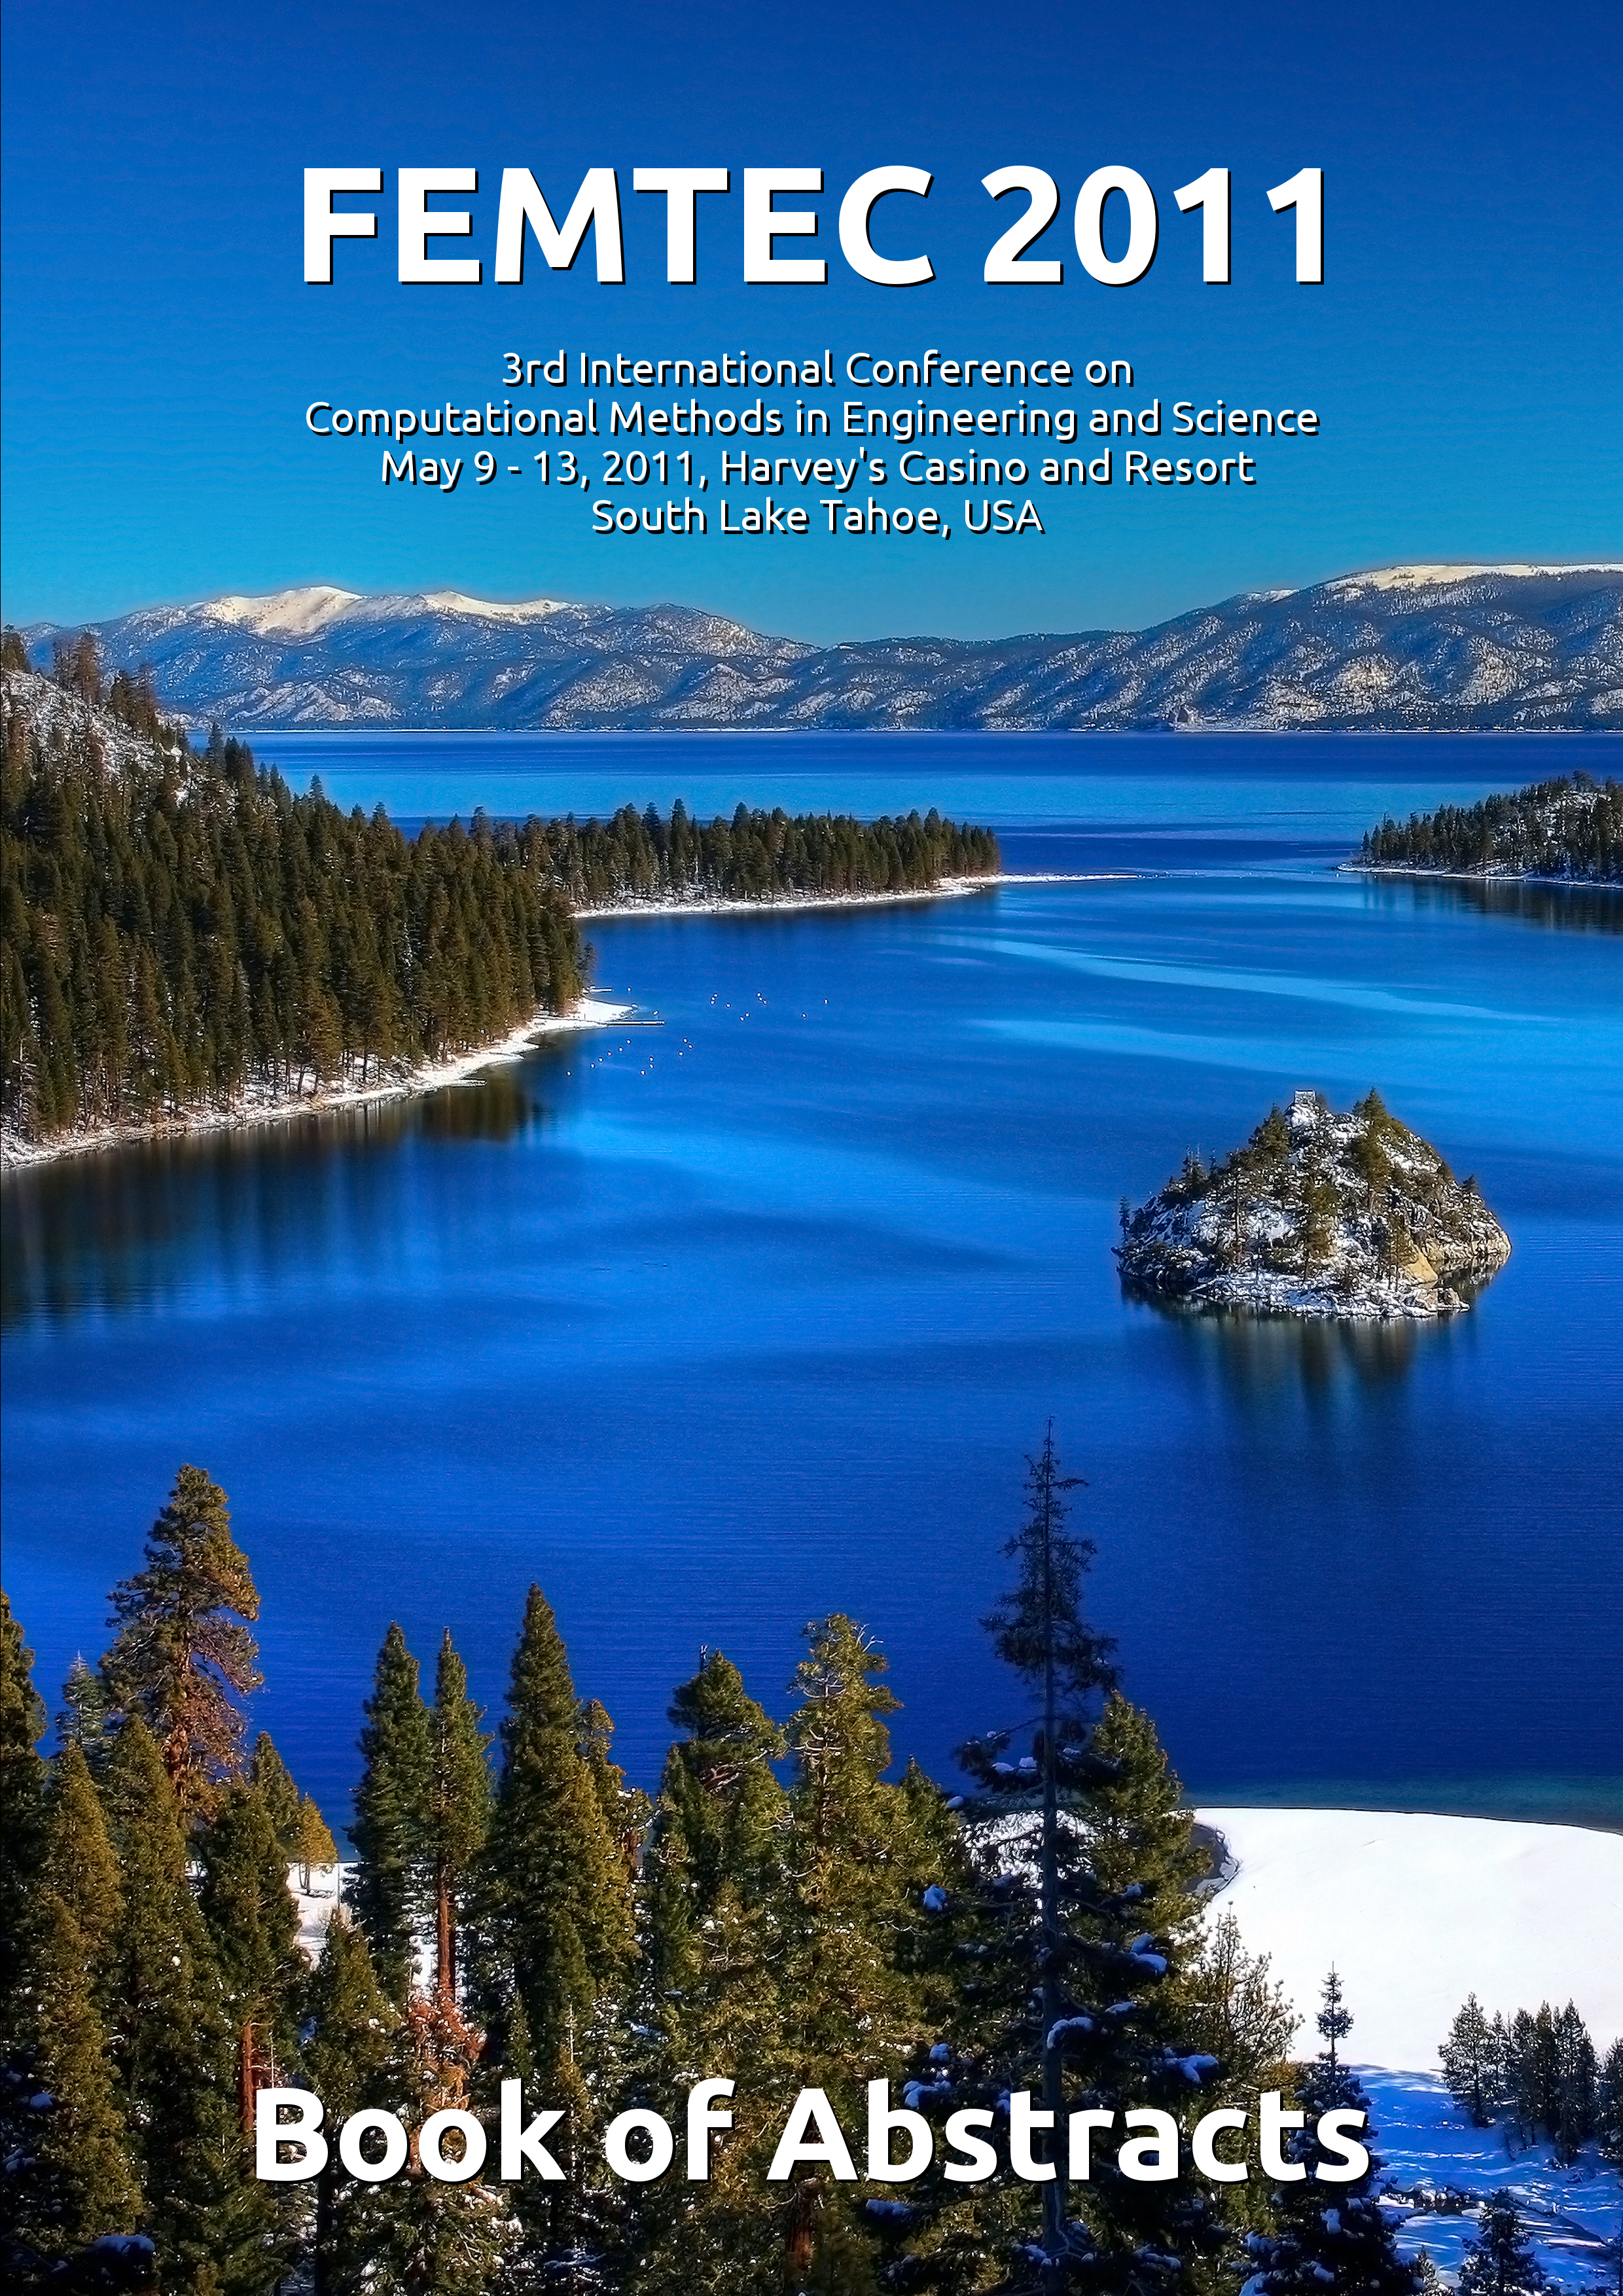
\includegraphics[width=\paperwidth,height=\paperheight]{img/background.jpg}
\vfill
}}}

\begin{document}

% INPUTTING BACKGROUND IMAGE
\AddToShipoutPicture{\BackgroundPic}
\vbox{}
\pagestyle{empty}
\newpage
\textwidth=15.5cm
\ClearShipoutPicture
\newpage

%%%%%%%%%%%%%%%%%%%%%%%%%%%%%%%%%%%%%%%%%%%%%%%%%%%%%%%%%%%%%%%%%%%%%%%%%

\section*{}
\small
\subsection*{About NCLab}
Networked Computing Laboratory (NCLab) is a popular Internet-based framework for 
programming, mathematics, computer modeling, 
and scientific computing. It serves students, instructors, researchers, and the general 
public. NCLab can be used free of charge for personal non-commercial purposes such as 
private hobby or self-education, as well as for individual non-funded academic research.
All other use is subject to {\bf purchasing a license} for a symbolic fee. The fees are as low as 
\$1 per user per month for educational use, and they are used to support the development 
and operational expenses. NCLab is a product of FEMhub Inc. The name "NCLab" is 
registered with the U.S. Patent and Trademark Office (USPTO) under Trademark No. 85420518.

\subsection*{Terms of Use and Pricing}
More details on purchasing a license and using NCLab are provided in the online documents 
{\bf Pricing} and {\bf Terms of Use} that are accessible from NCLab's home page 
{\tt http://nclab.com}.

\subsection*{Contact Information}
General inquiries: {\tt info@femhub.com}\\
Sales: {\tt sales@femhub.com}\\
NCLab support: {\tt support@nclab.com}\\
Agros \& Hermes support: {\tt support@femhub.com}\\
Web page: {\tt http://femhub.com}\\
{Physical address}\\
FEMhub Inc.\\
5490 Twin Creeks Dr.\\
Reno, NV 89523

\subsection*{About This Publication}
This publication can be copied and distributed without any restrictions
as long as reference to NCLab and FEMhub Inc. is preserved.


\normalsize

\newpage
%{\ }
\setcounter{tocdepth}{2}
\tableofcontents
%\pagestyle{plain}

\newpage

\pagestyle{plain}
\setcounter{page}{1}

%%%%%%%%%%%%%%%%%%%%%%%%%%%%%%%%%%%%%%%%%%%%%%%%%%%%%%%%%%%%%%%%%%%%%%%%%

\section{Introduction}

NCLab is a perfect place for instructors and students of Numerical Methods 
courses to experiment with the methods directly in classroom, as well as to 
complete / grade homework assignments. The list of programs that are readily 
available as Displayed Projects covers completely Numerical Methods I and 
Numerical Methods II, as these courses are taught at most colleges and 
universities. 

This tutorial does not discuss derivations and theoretical aspects of 
numerical methods. Instead, it describes the usage of programs 
that you can experiment with in order to complete your understanding 
of the theory. 

\section{Getting Started}

After entering NCLab at {\tt http://nclab.com}, you will see a desktop with several icons on it,
as shown in Fig. \ref{fig:desktop}. 

\begin{figure}[!ht]
\begin{center}
\includegraphics[width=\textwidth]{img/desktop.png}
\end{center}
%\vspace{-2mm}
\caption{NCLab desktop.}
\label{fig:desktop}
\vspace{-1cm}
\end{figure}
\newpage
\noindent
The function of these icons and a lot of other useful information for newcomers is provided 
in the introductory tutorial "Meet Your New Graphing Calculator" that is available in 
PDF via a link on NCLab home page. \\

\subsection{Cloning Displayed Projects}

All examples that we are going to work with in the following are also available 
as Displayed Projects. This means that you can clone them by launching the File
Manager, going to the {\em Project} menu, and clicking on {\em Clone}. This will launch 
a window with many displayed projects from various areas of programming,
math and computing. Look for projects whose names start with "Numerical Methods - 01",
"Numerical Methods - 02" and such.

After you locate a project that you would like to clone, click on it,
and then click on the button {\em Clone} at the bottom of the window. This will
create exact copy of that project in your account, and you can open it 
by clicking on it in the File Manager. You can change the project in any way 
you like, the changes will not affect the original Displayed Project. 


\subsection{Launching a new Python project}

For those who prefer to do the programming by themselves: 
In the File Manager's {\em Project} menu 
choose {\em New} $\rightarrow$ {\em Python}. This will launch an 
empty Python project, as shown in Fig. \ref{fig:python}.


\begin{figure}[!ht]
\begin{center}
\includegraphics[width=\textwidth]{img/python.png}
\end{center}
%\vspace{-2mm}
\caption{Launching a new Python project.}
\label{fig:python}
\end{figure}
\noindent

\newpage


\section{Warming Up}



\subsection{Finite computer arithmetic}

We start with a simple program that demonstrates that the computer 
arithmetic is finite. If the computer stored numbers exactly 
as we know them from mathematics, then the following program 
would run forever:

\begin{verbatim}
# Finite computer arithmetics.
eps = 1.0
while 1.0 - eps < 1.0:
    print "eps =", eps
    eps /= 10.
print "Boom!"
\end{verbatim}
However, the output looks as follows:

{\small
\begin{verbatim}
eps = 1.0
eps = 0.1
eps = 0.01
eps = 0.001
eps = 0.0001
eps = 1e-05
eps = 1e-06
eps = 1e-07
eps = 1e-08
eps = 1e-09
eps = 1e-10
eps = 1e-11
eps = 1e-12
eps = 1e-13
eps = 1e-14
eps = 1e-15
eps = 1e-16
Boom!
\end{verbatim}
}
\noindent
So, the computer can't distinguish between $1$ and $1 - 10^{-17}$!

\subsection{Absolute and relative error}




\subsection{Taylor polynomial}



\section{Solving Nonlinear Equations}




\subsection{Bisection method}



\subsection{Newton's method}

\subsection{Newton's method for systems}



\subsection{Fixed point method}


\subsection{Fixed point method with Anderson acceleration}

Anderson acceleration (sometimes called {\em Anderson mixing}) is a technique
to speed up the convergence of the fixed point method by considering 
a suitable linear combination of a few latest approximations, rather than 
just the latest approximation alone. 





\subsection{Solving polynomial equations with Numpy}





\section{Interpolation}





\subsection{Polynomial (Lagrange) interpolation}




\subsection{Interpolation with cubic splines}



\section{Matrix Methods}



\subsection{Dense and sparse matrix}


\subsection{Singular, nonsingular and inverse matrix}


\subsection{Condition number}


\subsection{LU factorization}


\subsection{Cholesky decomposition}


\subsection{Jacobi method}


\subsection{Gauss-Seidel method}


\subsection{SOR method}


\subsection{Steepest descent method}


\subsection{Modern iterative methods}


\subsection{COO to CSR conversion}


\subsection{CSR matrix-vector multiplications}


\subsection{Moore-Penrose inverse}




\section{Numerical Quadrature}


\subsection{Piecewise constant}


\subsection{Trapezoidal rule}


\subsection{Simpson's rule}


\subsection{Calculating weights}


\subsection{Arbitrary interval}


\subsection{Getting Gauss points and weights from Scipy}


\subsection{Gauss quadrature with $n$ points}


\subsection{Adaptive Gauss Quadrature}



\section{Approximation}


\subsection{Nonlinear regression}


\subsection{Linear regression}

\subsection{Least squares fit (continuous case)}


\subsection{Fourier series expansion}



%\begin{figure}[!ht]
%\begin{center}
%\includegraphics[width=0.8\textwidth]{img/temple0.png}
%\end{center}
%\vspace{-2mm}
%\caption{Sample PLaSM model (available as Displayed Project "Temple").}
%\label{fig:pisa}
%\end{figure}



\end{document}
